\section{Platform Overview}

\begin{figure}[h]
  \centering
  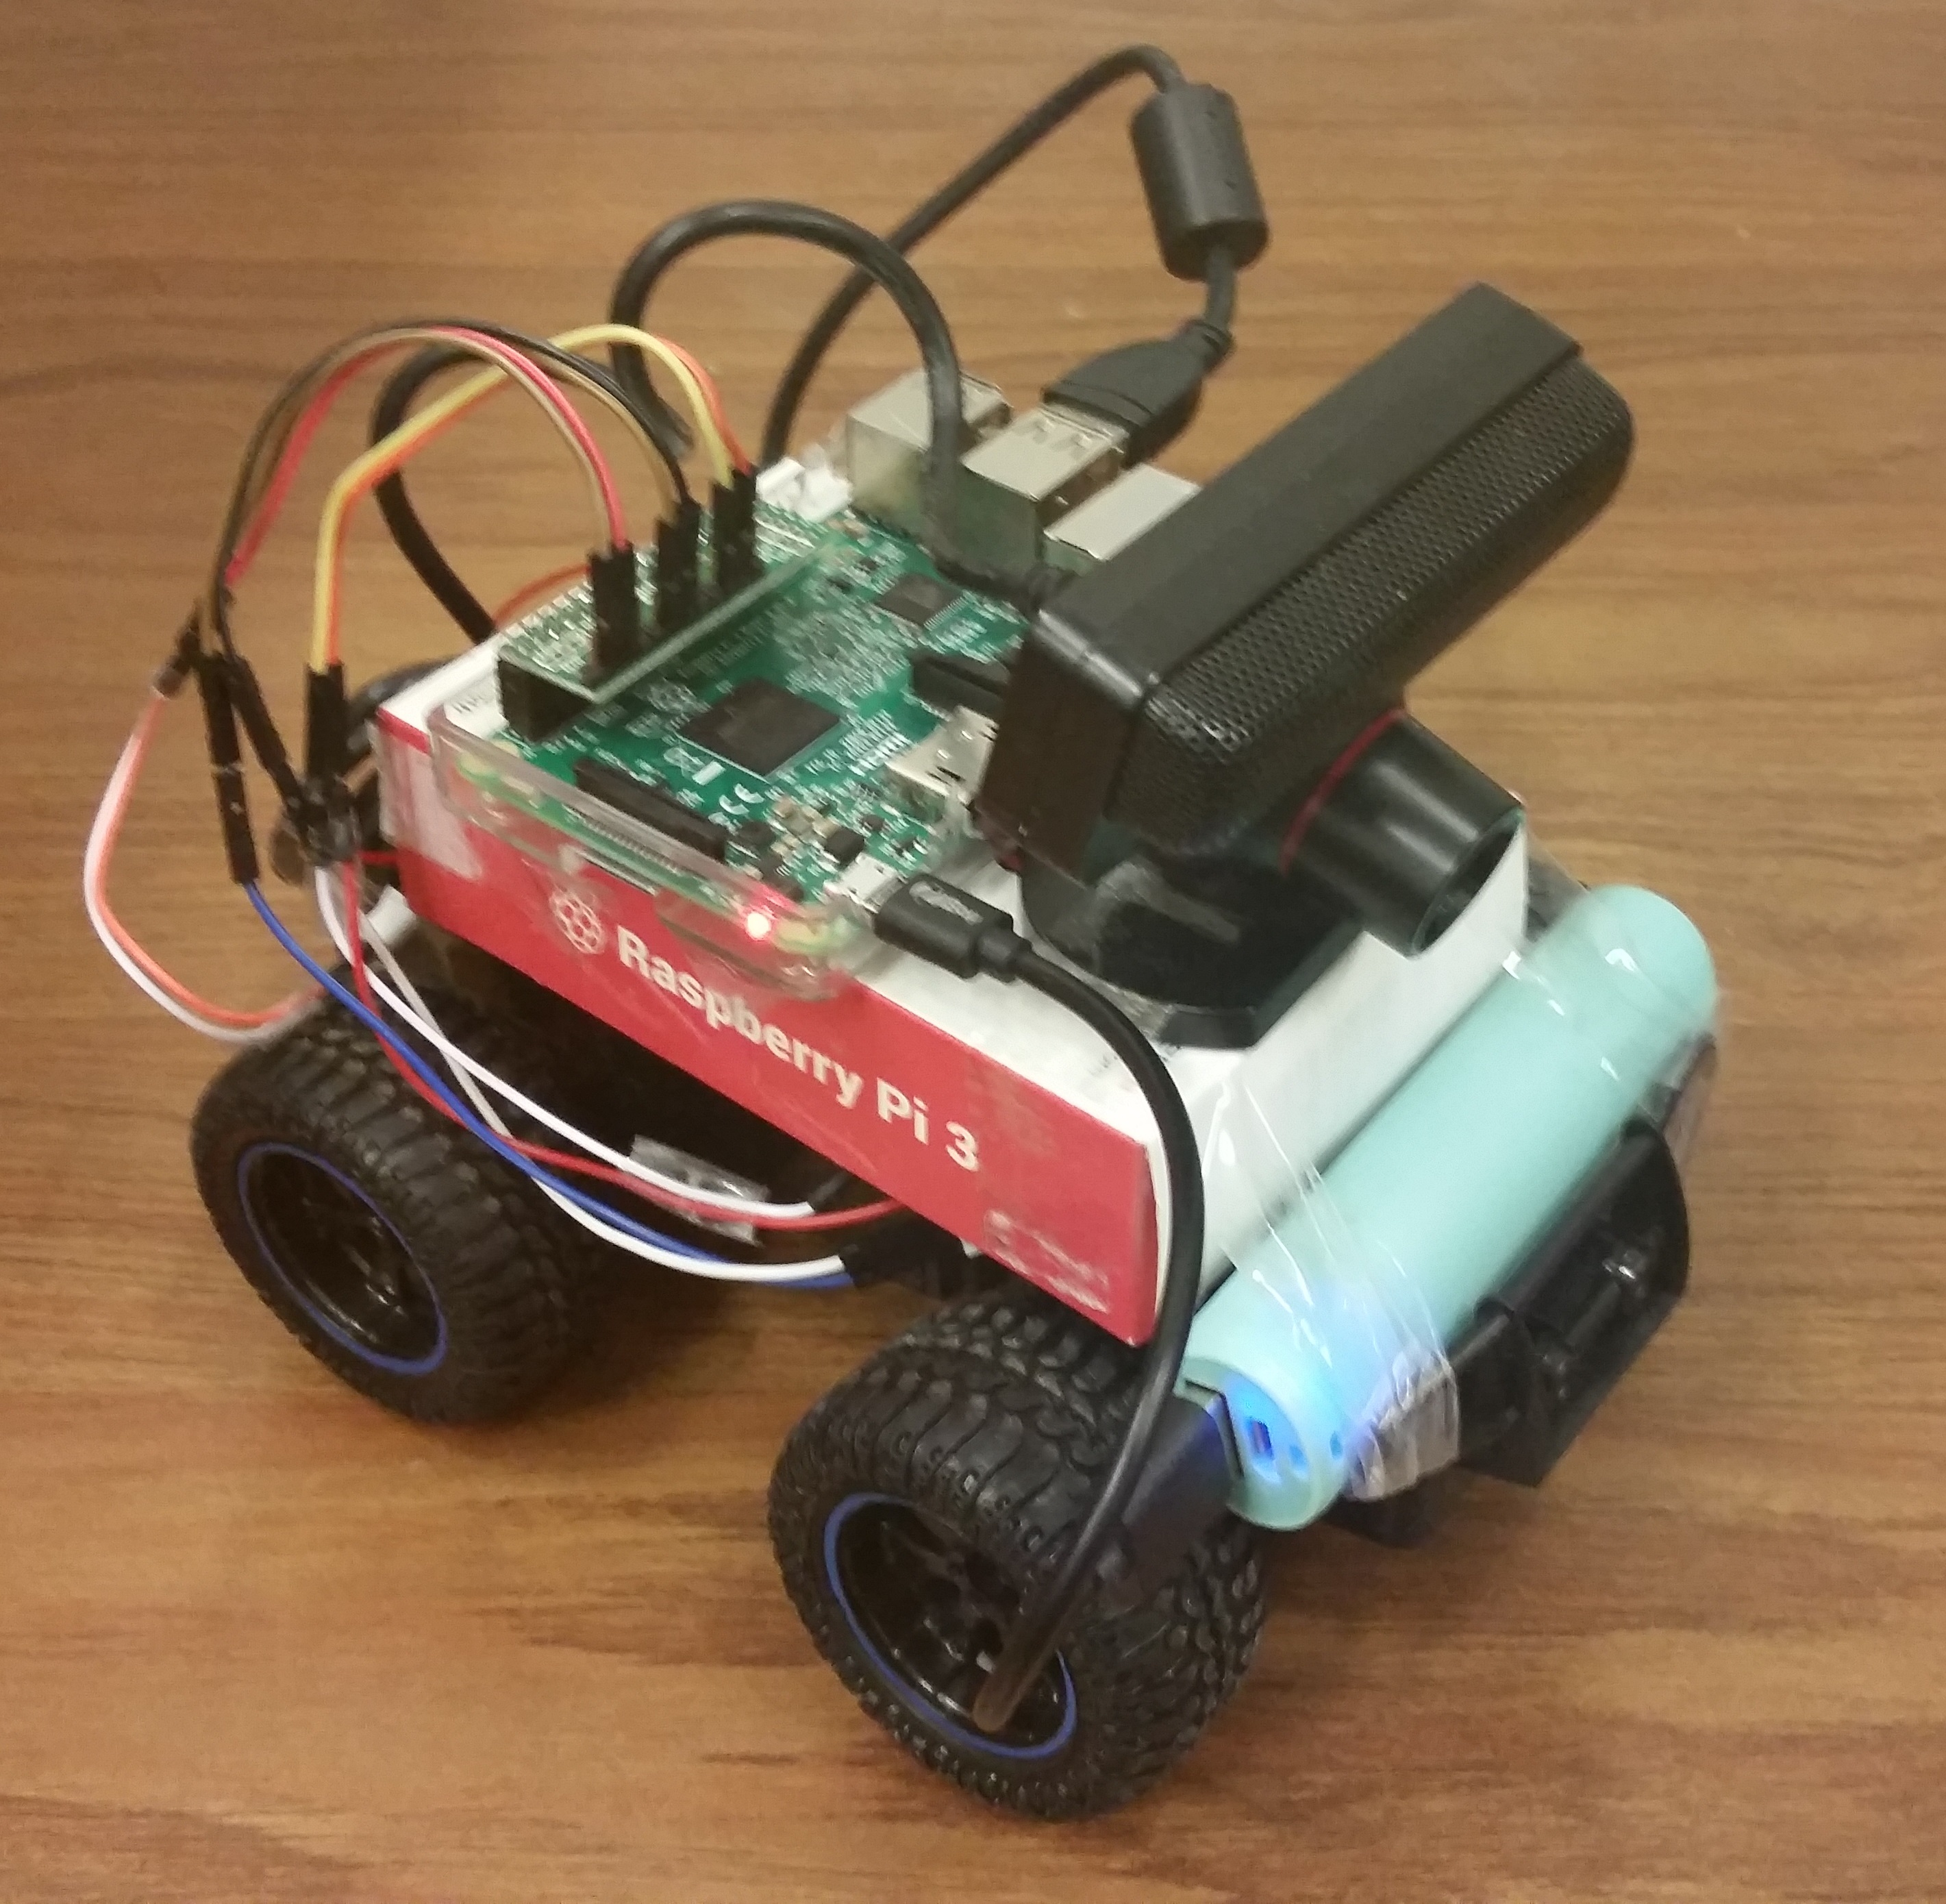
\includegraphics[width=.4\textwidth]{Picar_Picture}
  \caption{ The Picar Platform. }
\end{figure}

\subsection{Platform Components}

\begin{table*}[h]
  \centering
  \begin{tabular} {| l | l | l | l | l |}
    \hline
    \textbf{Platform} & \textbf{Picar} & \textbf{F1/10} & \textbf{NVIDIA DAVE-2}\\ \hline 
    Car & Mini RC Car (\$10) & Traxxas 1/10th car platform (\$299.97) & TBD\\ \hline
    Embedded system & Raspberry Pi 3 Model B (\$35.00) & NVIDIA Jetson TK1 (\$192.99) & NVIDIA DRIVE PX \\ \hline
    CPU & Cortex A-53 quad core & Cortex A-15 quad core & 8x Cortex A-57 quad core, 8x Cortex A-53 quad core \\ \hline
    Camera & Playstation Eye camera (\$6.99) & ZED camera (\$449.00) & 3x cameras\\ \hline
    Power Supply & Mobile battery (\$5.99) & Energizer battery pack (\$159.00) & TBD\\
    \hline
  \end{tabular}
  \caption{Comparison of components used in autonomous vehicle platforms.}
\end{table*}

We employ a small and relatively inexpensive RC car that is capable of performing basic automotive 
operations. However, the car we use doesn't replicate the capabilities of other autonomous vehicle 
platforms, as it is more simplistic in nature. Notably, the RC car we use only has three possible 
options in terms of turning: center, left, and right. As such, control of the car may be less precise at 
times, and may negatively affect performance. The car is capable of other operations that aren't used 
within the scope of this platform. Specifically, the car is able to drive in reverse and the driving 
speed can be changed. In our experiments, we have the RC car drive forward, and at a constant speed.

Our platform also comes equipped with a camera that is used for both recording training videos and 
providing input frames to the model whenever the Picar is self-driving. We chose the Playstation Eye 
Camera due to its ability to reach and maintain higher fps levels while also remaining relatively 
low-cost. One concern, however, is the affect of camera latency on the self-driving performance of our 
platform. While humans are able to see environmental changes in real-time, the same can't be said for 
cameras since there is a delay between when frame capture by the camera, and when it is read by the 
Raspberry Pi 3. As a result, it is possible for the model to be given an input frame that is different 
from the real world, thus impacting the performance of the Picar.

Compared to other existing autonomous vehicle platforms, such as the F1/10 and NVIDIA DAVE-2, the Picar 
platform is capable of performing the same operations while using more cost inexpensive components. As 
shown by Table 1, the components selected for the Picar all cost considerably less than the other 
platforms when focusing on the common components (camera, power supply, etc.). Including the other 
components used in the F1/10 and DAVE-2, such as the additional sensors employed by both, the difference 
in cost would be even greater.

\subsection{Model Training}
In order to operate the Picar as an autonomous vehicle, we utilize the DeepTesla library, which is 
capable of training a deep neural network (DNN) with end-to-end learning, that could then be used by the 
Picar for autonomous driving. Please note that it is more efficient to execute the actual model training 
process on a different system with an NVIDIA GPU, rather than on the Raspberry Pi 3 itself. This is 
because DeepTesla trains the DNN with the Tensorflow library, which greatly benefits from the use of 
gpu-enabled operations. For comparison, training a model on the Pi took approximately 6 hours, whereas 
the time it took on a computer with a NVIDIA GPU was only around 5 minutes! 

We train our model on a custom made track/lane composed of black and white duct tape, where the black 
tape represents the bounds of the track, and the white tape marks the center of the lane. The model is 
taught to stay close to the center of the lane for as long as possible, and to turn whenever it 
reaches/crosses the outer lane bounds so that it remains on the track. For data, we navigate and record 
the car going both ways across the track, and use the collected videos to train the model(s) that will 
be used later for angle prediction while the car is self-driving.

